\section{Minimalist Prover}

\subsection{Research}
\begin{frame}{Minimalist Prover: Motivation}
	\begin{itemize}
		\item Prover is the final phase of the verification pipeline
		\item Sole determiner of which VCs can or can not be automatically proved
		\item Nearly all verification efforts focused on more efficient provers
		\item Our hypothesis suggests that, in many cases, \emph{flexibility} may trump raw performance
	\end{itemize}
\end{frame}

\begin{frame}{Minimalist Prover: Contributions}
	\begin{itemize}
		\item We demonstrate how a number of components can be engineered in a rigorous style to ease the verification process
		\item We experiment with a suite of prover heuristics intended to expose the programmer's underlying logic
		\item We confirm empirically that well-designed components built on an expressive mathematical framework can be dispatched by a minimalist prover
		\item Among these components, we present a mechanically verified generic sorting algorithm---a first
		\item For full details, see Chapter 7
	\end{itemize}
\end{frame}

\begin{frame}{Minimalist Prover: Design}
	\begin{itemize}
		\item Simple rewrite prover
		\item New features only when justified by VCs from real verification problems
		\item Flexible for experimentation
		\item Data collection for comparison
		\item Pedagogical deployments
	\end{itemize}
\end{frame}


\begin{frame}{Demo: Flipping a Queue}
~
\end{frame}

\begin{frame}{Demo: Flipping a Queue}
\centering{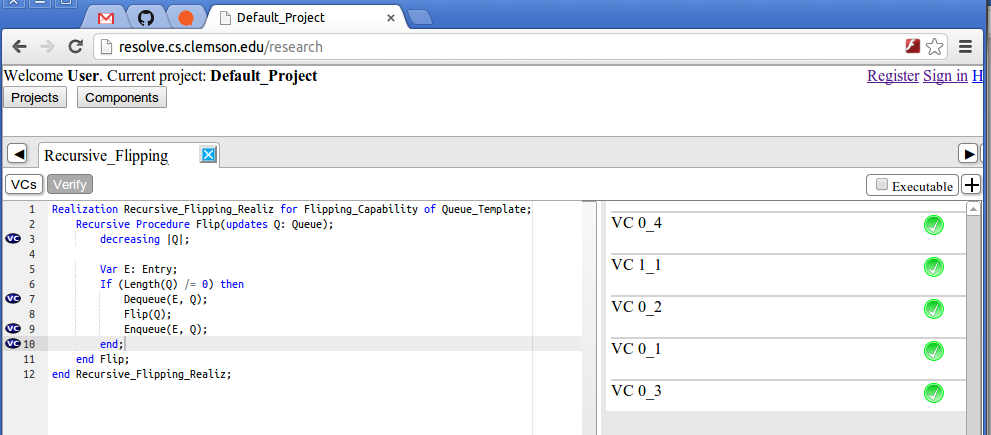
\includegraphics[width=\textwidth]{works}}
\end{frame}

\begin{frame}{Demo: Flipping a Queue}
\centering{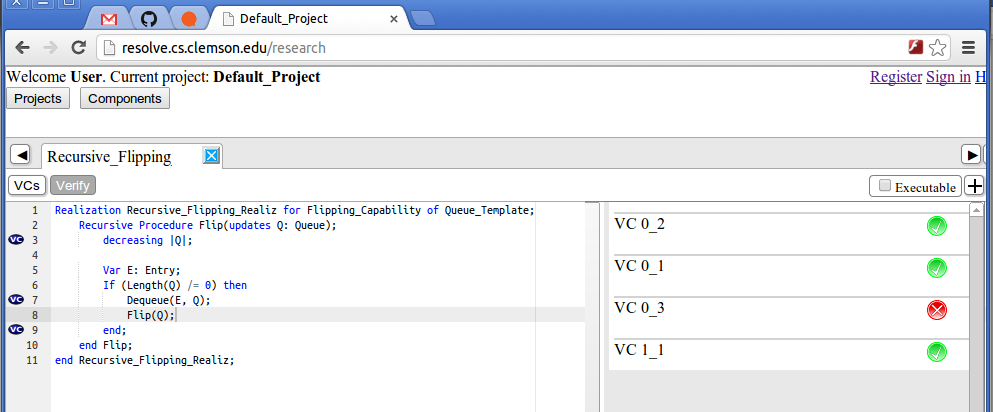
\includegraphics[width=\textwidth]{doesnotwork}}
\end{frame}


\begin{frame}{Automated Prover Algorithm}
	\begin{enumerate}
		\item Expand variables\\
			\texttt{i = j - 1}
		\item Develop antecedent\\
			\texttt{A and (A implies B) implies B}
		\item Explore consequent\\
		\begin{itemize}
			\item Tethered depth-first search\\
				Prevents \texttt{i < j implies i < j + 1} or \texttt{Reverse(Empty\_String) = Empty\_String} from being applied ad nausium
			\item Terminates when proof space is exhausted or all consequents are dispatched
		\end{itemize}
	\end{enumerate}
\end{frame}


\begin{frame}{Automated Prover Algorithm}
	\begin{itemize}
		\item Extremely straightforward
		\item Similar to how a human mathematician might perform a proof
		\item Many irrelevant antecedent developments are likely to be made
		\item Antecedent development happens once, up-front, so time is less of an issue, but space complexity is combinatorial
		\item During consequent exploration, full proof space must be searched.  Combinatorial time complexity is a problem.
	\end{itemize}
\end{frame}


\begin{frame}{Automated Prover Algorithm: Heuristics}
	\begin{itemize}
		\item Detect and avoid useless transformations\\
			\texttt{S} $\rightarrow$ \texttt{S o Empty\_String}
		\item Develop only about relevant terms\\
			\texttt{f(a) and g(b) implies h(b)}
		\item Diversify givens
		\item Minimize as a preprocessing step
		\item Detect cycles
		\item Prioritize transformations as a preprocessing step\\
			\begin{enumerate}
				\item Reduce unique symbols
				\item Reduce function applications
			\end{enumerate}
	\end{itemize}
\end{frame}


\subsection{Evaluation}
\begin{frame}{Experimental Evaluation: Overview}
	\begin{itemize}
		\item Questions\\
		\begin{itemize}
			\item Is such a minimalist prover practical?
			\item Are the heuristics effective?
		\end{itemize}
		\item Approaches\\
		\begin{itemize}
			\item Series of verification benchmarks over multiple domains: integers, arrays, queues, trees
			\item Collect metrics
			\item How effective is the prover at dispatching VCs in a reasonable amount of time?
			\item What causes VCs not to prove?
			\item How does disabling each heuristic impact verification metrics?
		\end{itemize}
		\item For full details, see Chapter 7
	\end{itemize}
\end{frame}


\begin{frame}{Experimental Evaluation: Metrics}
	\begin{itemize}
		\item VCs proved
		\item Real time
		\item Operative steps
		\item Search steps (subset of operative steps occurring during consequent exploration)
	\end{itemize}
\end{frame}


\begin{frame}{Sorting a Queue}
	Specify a user-defined FIFO queue ADT that is generic (i.e., parameterized by the type of entries in a queue). Verify an operation that uses this component to sort the entries in a queue into some client-defined order.
	\vspace{2em}
	\lstinputlisting[language=resolve,caption=]{examples/Sorting_Capability_bad.en}
\end{frame}


\begin{frame}{Sorting a Queue}
	Specify a user-defined FIFO queue ADT that is generic (i.e., parameterized by the type of entries in a queue). Verify an operation that uses this component to sort the entries in a queue into some client-defined order.
	\vspace{2em}
	\lstinputlisting[language=resolve,caption=]{../proverEval/examples/Sorting_Capability.en}
\end{frame}


\begin{frame}{Sorting a Queue}
	\lstinputlisting[language=resolve,caption=]{examples/Selection_Sort_Realization1.rb}
\end{frame}


\begin{frame}{Sorting a Queue}
	\lstinputlisting[language=resolve,caption=]{examples/Selection_Sort_Realization2.rb}
\end{frame}


\begin{frame}{Sorting a Queue}
	\begin{itemize}
		\item VCs proved: 16/16
		\item Mean time: 1781 ms
		\item Median operative steps: 8
		\item Median search steps: 0
	\end{itemize}
	\centering{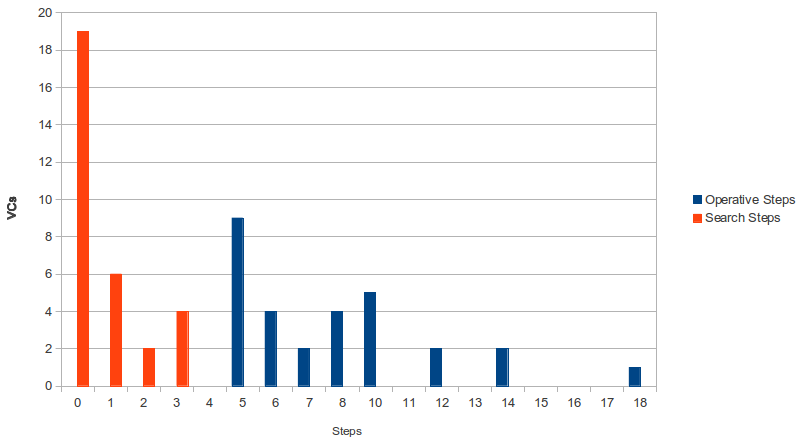
\includegraphics[width=.8\textwidth]{QueueSortHist}}
\end{frame}


\begin{frame}{Demo: Array Realization of a Stack}
~
\end{frame}


\begin{frame}{Array Realization of a Stack}
	Specify a user-defined LIFO stack ADT that is generic (i.e., parameterized by the type of entries in a queue). Verify an array implementation of that ADT.
\end{frame}


\begin{frame}{Array Realization of a Stack}
	\lstinputlisting[language=resolve,caption=]{../proverEval/examples/Stack_Template.co}
\end{frame}


\begin{frame}{Array Realization of a Stack}
	\lstinputlisting[language=resolve,caption=]{examples/Array_Realiz.rb}
\end{frame}


\begin{frame}{Array Realization of a Stack}
	\begin{itemize}
		\item VCs proved: 27/27
		\item Mean time: 1707.1 ms
		\item Median operative steps: 6
		\item Median search steps: 0
	\end{itemize}
	\centering{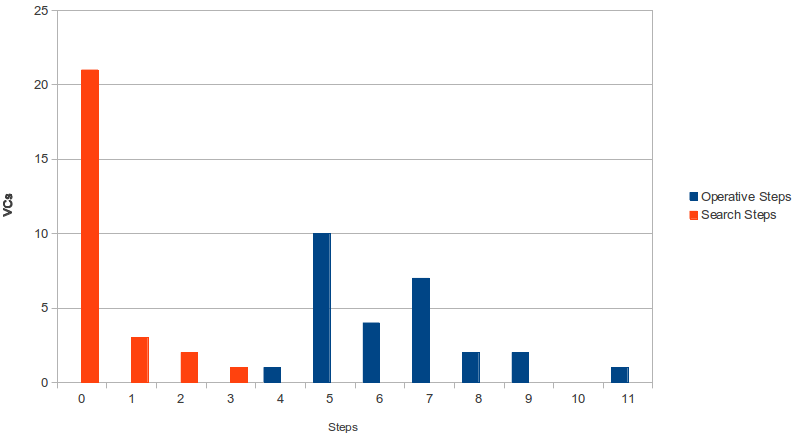
\includegraphics[width=.8\textwidth]{ArrayRealizHist}}
\end{frame}


\begin{frame}{Overall Experimentation Results}
	\begin{itemize}
		\item Six representative examples over integers, arrays, stacks, queues, and trees:\\
		\begin{itemize}
			\item Add/Multiply Integers
			\item Binary Search Array
			\item Sort a Queue
			\item Flip a Queue
			\item Array Implementation of Stack
			\item Modify and Restore a Tree
		\end{itemize}
		\item VCs proved: 127/133
		\item Mean time: 2493 ms
		\item Median operative steps: 7
		\item Median search steps: 0
	\end{itemize}
\end{frame}


\begin{frame}{Overall Experimentation Results}
	\begin{figure}
		\centering
		\begin{subfigure}[b]{0.40\textwidth}
			\centering
			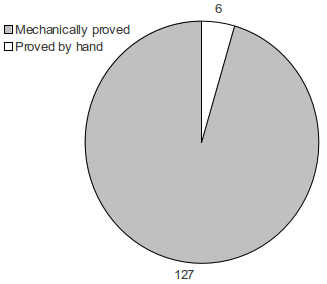
\includegraphics[width=\textwidth]{../proverEval/proofResults3.png}
			\caption{Verification results\label{fig:pie}}
		\end{subfigure}
		\quad
		\begin{subfigure}[b]{0.55\textwidth}
			\centering
			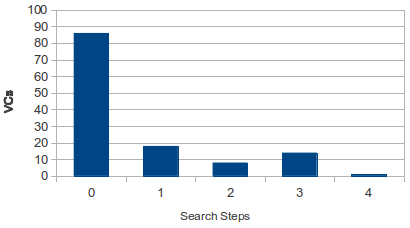
\includegraphics[width=\textwidth]{../proverEval/searchSteps2.png}
			\caption{Number of Search Steps Required by Proofs\label{fig:histogram}}
		\end{subfigure}
	\end{figure}
\end{frame}


\begin{frame}{Heuristic Evaluation}
	\tiny
	\begin{tabular}{lrrrrrrr}
		\toprule
			& $\sum \Delta\text{Proved}$	& $\overline{\Delta t / \sigma}$	& $\sum\Delta t$ & $\overline{\Delta\text{steps}}$ & $\sum\Delta\text{steps}$ & $\overline{\Delta\text{search}}$ & $\sum\Delta\text{search}$ \\
		\midrule
		With useless \\
		transformations		& -12	& 4.07	& 83438		& 0	& 0	& 0	& 0	\\
		\midrule
		Developing about \\
		irrelevant terms	& -1	& 8.80	& 154530	& 0	& 0	& 0	& 0\\
		\midrule
		Not checking for \\
		diversity of givens	& -6	& -5.55	& -142026	& -0.02	& -4	& -0.01	& -1	\\
		\midrule
		No minimization		& -10	& 2.53	& 36651		& 0.02	& 3	& 0.28	& 35	\\
		\midrule
		No cycle detection	& 0	& 0.60	& 9629		& 0.08	& 11	& 0.08	& 11	\\
		\midrule
		No prioritization \\
		of transformations	& -19	& 2.60	& 17577		& 0.05	& 6	& 0.04	& 5	\\
		\bottomrule
	\end{tabular}
\end{frame}
